\section{Introduction}
\setcounter{page}{1}
\pagenumbering{arabic}

During this age of space-born solar astronomy, understanding the highly dynamic environment of the Sun's atmosphere is a study enriched by a wealth of high detail observations. With each newly launched space instrument the spatial resolution of collected data increases, which coupled with those spacecraft that are tailored to capture light of previously unobserved wavelengths, often leads to new phenomena being observed. Eruptive solar flares fall into this category, in that spacecraft have provided observations that challenge the current theoretical view that the standard eruptive flare model (CSHKP model: \citep{1964NASSP..50..451C, 1966Natur.211..695S, 1974SoPh...34..323H, 1976SoPh...50...85K} puts forward.

Solar flares are one of the most energetic events to occur in the Sun's atmosphere, where by stored magnetic energy is released in the form of heat, mass motions, and accelerated particles. This highly dynamic process produces many measurable emission signatures at wavelengths from $\gamma$-rays to radio waves. Many of these observed signatures agree with the CSHKP model, however, this is not the full picture. The standard flare model has been modified to include new observations many times over the years (e.g., \cite{2011LRSP....8....6S}) and is still unable to describe some observed phenomena. 

Sunquakes are an observable feature (shown in Figure \ref{mdiquake96}) during some solar flares that the standard model is unable to explain. It is believed that they are the result of energy and momentum released during the flare impacting the lower solar atmosphere. If a sufficient amount of momentum is imparted on the lowest atmospheric layer, then acoustic waves or 'sunquakes' are produced. The challenges presented in studying this phenomena are mainly associated with the ambiguous nature of the mechanism by which sunquakes are generated. Many ideas for the sunquakes progenitors have been put forward but at this point in time observable signatures do not always show a clear cut evidence aligning with current theories. Therefore this is an exciting time to be investigating the formation mechanisms of sunquakes and could also contribute to our overall understanding of solar flares. 

This work is focused on the determination of the sunquake generation mechanism for the X-class solar flare on the 29th of March 2014. The main emphasis being on whether two of the proposed sunquake progenitors (see section \ref{sunprog}), namely direct particle beam collision and radiative backwarming, leave an energy deposition signature comparable in magnitude to the acoustic impact power at the epicentre of the seismic disturbance.      


%%%%%%%%%%%%%%%%%%%%%%%%%%%%%%%%%%%%%%%%%%%%%%%%
%%%%%%%%END OF SOFT INTRO%%%%%%%%%%%%%%%%%%%%%%%


\subsection{Eruptive Solar Flares}\label{flares}

Solar flares are the explosive conversion of magnetic energy into mass motions, radiation, electric currents and MHD waves. These events are the most energetic of solar phenomena and can be observed throughout the entire solar atmosphere, with some of the larger flares releasing up to $10^{37}$ erg of energy. Flares are classified by the the Geostationary Operational Environmental Satellite (GOES) see Table \ref{goes}, in this stem, the logarithmic measure of 1 to 8 \AA\ X-ray flux produced by the flare determines it's classification. The GOES system classes flares from X to A-class, in order of high to low flux, so an X-class flare event would be more powerful than an M-class and so on. \\

\begin{table}[h]
\centering
\begin{tabular}{|c|c|}\label{GOES}
Classification & Peak Flux Range at 1 to 8 \AA\ ($W.m^{-2}$) \\
\hline
X & $10^{-3}$ - $10^{-4}$\\
M & $10^{-4}$ - $10^{-5}$\\
C & $10^{-5}$ - $10^{-6}$\\
B3 & $10^{-6}$ - $10^{-7}$\\
A & $<10^{-7}$\\
\end{tabular}
\caption{shows the GOES flare classification, which is based on the order of magnitude of hard x-ray flux. X class flares produce a flux of $10^{-3}$ - $10^{-4}$ $W.m^{-2}$ and are the most powerful, whilst a weak A class flare can produce less than $10^{-7}$ $W.m^{-2}$.}\label{goes}
\end{table}

\subsubsection{Standard Eruptive Flare Model}
The standard solar flare theory, also known as the CSHKP model, is the culmination of research by many authors,\citep{1964NASSP..50..451C, 1966Natur.211..695S, 1974SoPh...34..323H, 1976SoPh...50...85K}, describing the formation and evolution of two-ribbon flares. 

\begin{figure}[H]
  \begin{center}
  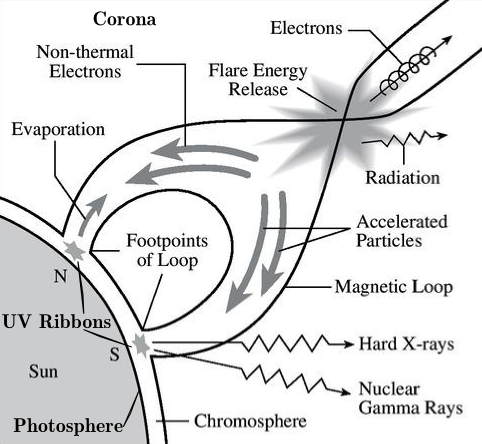
\includegraphics[width=0.40\textwidth]{flare}
  \caption{cartoon of the standard 2D solar flare model. Image courtesy of \href{http://ase.tufts.edu/cosmos/print_images.asp?id=47}{www.tufts.edu}}\label{flare-cartoon}
\end{center}
\end{figure}
 

In this model, a flux tube tethered to the photosphere, has expanded into the corona forming a loop. These extended magnetic loops can become stressed by processes such as convective motions, differential rotation, flux emergence and sun-interplanetary MR. The stressing of a magnetic field is a method of storing magnetic free energy, which can be released via reconnection which reconfigures the magnetic field to a lower (potential) energy state. In the standard eruptive flare model, magnetic free energy is stored high up in the corona, built up by a filament rising through the atmosphere. A filament is cool dense plasma suspended in the corona overlying an active region's polarity inversion line \citep{1955ApJ...121..349B}. It is thought that filaments are suspended up in the corona by magnetic fields in the form of either a sheared arcade or a flux rope which is the focus of the CSHKP model. As the filament (flux rope) rises, it drags the surrounding magnetic loops along with it, which creates a situation where the legs of the loops start to flow inward. As this inward flow causes opposing magnetic legs to get closer to each other, a current sheet develops which stretches along the neutral region. This current sheet eventually becomes thin enough that magnetic reconnection occurs due to a decreased scale-length $l$. This means that conductivity drops and electric currents are suddenly able to dissipate. This causes the time derivative of the magnetic field (induction equation \ref{MHD}) to be dominated by the diffusion term, at which point, magnetic flux will break out of the frozen-in condition and MR can occur. The location where reconnection happens is known as a magnetic null. Considering the 2D case, the magnetic null takes on an 'X' type structure whereby two in-flowing magnetic field lines reconnect to form two out-flowing magnetic field lines. Inflowing magnetic field reconnects in the diffusion region with a configuration of increased magnetic tension or curvature, which drives post-reconnection outflow of the newly connected field. This process reconfigures the magnetic field from an expanding loop with inflowing legs to outflowing flare loop and filament structure. At the point of reconnection, energy is released in the form of heating, accelerated particles and MHD waves. Heating can reach temperatures of $10^7$ K and accelerated particles travel down flare loops causing emission, shocks and sometimes acoustic disturbances in the solar interior or sunquakes. The appearance of two flare ribbons is caused by reconnection occurring simultaneously across an arcade of magnetic loops. Accelerated particles travel down each loop in the arcade, colliding with the chromosphere as they do, at which point bremstrahlung and H$\alpha$ emission are produced, leading to the appearance of footpoints and ribbons respectively. A cascade of these reconnection events occur as the erupting filament rises through each successive loop making up the overlying non-potential magnetic field. When applied to the entire arcade of loops making up the field this leads to the appearance of flare ribbons moving outward from the polarity inversion line. If a filament is not present, \cite{2005psci.book.....A} describes the build up of magnetic free energy as being caused by the evolution of the associated active region, whereby photospheric plasma motions shear the magnetic field arcade causing reconnection. 


\subsubsection{Solar Atmosphere}
For a sunquake to occur, energy released during a solar flare has to traverse four layers of the solar atmosphere, known as the corona, transition region, chromosphere and photosphere. Each region is very different in terms of plasma density meaning energy and momentum have to navigate multiple pressure scale heights. Pressure scale height, $H$, is a measure of the distance over which pressure drops off by a factor of \emph{e}. For example, in the photosphere, $H\sim150$km, whereas in the corona, $H\sim100$Mm. This means that in the photosphere, pressure and density are changing rapidly, making it increasingly likely that energy deposition via heat conduction, particle collisions and shocks will occur. Figure \ref{solatm} shows how temperature and density in each layer of the solar atmosphere change with height. \\

The photosphere is the region where sunquakes manifest as observable concentric circular waves, emanating from a central impact zone, shown in Figure \ref{mdiquake96}. The lowest in altitude of the atmospheric layers, the photosphere forms a shell around the Sun with a radius somewhere between $\sim10$ - $10^{2}$ km, with an effective temperature of $T\sim5800$K and decreasing in temperature with radial distance to $\sim4400$K at the temperature minimum region, see figure \ref{solatm}. Emission from this part of the atmosphere is predominantly in the visible range. The densest atmospheric layer, plasma pressure in the photosphere is dominant over magnetic pressure such that the plasma-beta, $\beta = p_{gas}/p_{mag} >> 1$. Active regions on the photosphere contain sunspots, which are regions of intense magnetic field playing host to footpoints of loops that can extend out into the corona. A sunspot is an approximately circular feature, made up of two main parts, the dark central umbra which is surrounded by the slightly lighter penumbra. The umbra hosts magnetic field lines that are tightly packed and pointing radially away from the Sun, whereas the penumbral magnetic field is more horizontal with respect to the solar surface. With a field strength of $\sim 10^{-1}$ Tesla, sunspots are regions in the photosphere where the magnetic pressure is dominant over plasma pressure, such that $\beta << 1$. Meaning that in these regions convection currents and radiative transfer are inhibited, with the latter being the idea behind a sunspot's dark appearance. \\



\begin{figure}[H]
  \begin{center}
    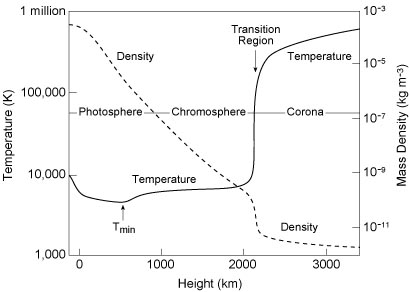
\includegraphics[width=0.5\textwidth]{solar-atm-plot}
\caption{The temperature of the solar atmosphere decreases from values near 6,000 degrees Kelvin at the visible photosphere to a minimum value of roughly 4,400 degrees Kelvin about 500 kilometres higher up. The temperature increases with height, slowly at first, then extremely rapidly in the narrow transition region, less than 100 kilometres thick, between the chromosphere and corona, from about $10^{4}$K to about $10^{6}$K. (Courtesy of Eugene Avrett, Smithsonian Astrophysical Observatory.)}\label{solatm}
  \end{center}
\end{figure}


The next region of the atmosphere is the chromosphere which is situated above the photosphere. Proposed sunquake generation methods (see section \ref{sunprog}) that involve the flow of momentum through the chromosphere are shocks, radiative backwarming and direct particle collision. These progenitors would have to be able to minimise the dissipative effects of the ever increasing plasma density throughout this region to produce a sunquake. Either that or the transfer of energy happens in such a way that the transport continues downward eventually reaching the photosphere. The chromosphere is a few thousand kilometres (2000 - 3000 km) thick and is optically thin to visible light so is difficult to observe against the brightness of the photosphere. The temperature in this layer increases with height from 4400 K at the temperature minimum region to $\sim10^{5}$K near the transition region. As a result, plasma density decreases and $\beta$ drops, crossing unity near the transition region between the upper-chromosphere and corona. This means that the pressure scale height in this region is changing with altitude as a transition from the plasma to magnetic domain occurs. Up in altitude to the interface between the chromosphere and the corona or transition region. This region is a poorly understood layer of the solar atmosphere. What is known, is that; temperatures climb from $\sim10^{5}$ near the chromsphere to $\sim10^{6}$ K at the corona; this region has variable thickness and maybe even orientation; plasma density falls off sharply. The corona is the outer most layer of the solar atmosphere, extending out into interplanetary space. This part of the atmosphere is threaded with expanded and stressed magnetic loops which are tethered at the photosphere. Stressed coronal loops store vast amounts of energy in the form of electric current, which can be released during a solar flare. At which point, energy and momentum are filtered down into deeper layers of the atmosphere, sometimes reaching all the way down to the photosphere and causing a sunquake. With a temperature ranging from $T\sim10^{6}$ - $10^{7}$ K, this the hottest part of the atmosphere. Plasma density in this region is very low, leading to a plasma pressure which is much lower than the magnetic pressure resulting in $\beta << 1$. This means that plasma motions are dominated by magnetic fields leading to magnetic loops that can expand almost unhindered. Information in this section is taken from text books: \cite{2003dysu.book.....D, 2004soas.book.....F}


\subsubsection{Energy Transfer}
The impulsive phase of a solar flare occurs when energy near the reconnection X-point is transported along the magnetic field into the chromosphere. The two basic methods of energy transport during this phase are thermal and non-thermal. In the thermal case, plasma in the top of a flare loop is heated by MR or shocks. In the non-thermal case, particles are imparted enough energy to no longer be described by the thermal Maxwellian distribution, instead exhibiting nonthermal energies. The energy source for nonthermal particles is thought to be MR. During the impulsive phase of a flare, electrons are accelerated to high energies, down newly reconfigured flare loops. These high energy electrons are fed into the dense plasma of the chromosphere and photosphere where they deposit their energy. The collisional thick target model by \cite{1971SoPh...18..489B} says that almost all of the flare energy is carried by the particle beam, therefore, energy dissipated in the lower atmosphere represents a large portion of the flare energy budget.

\subsubsection{Thick Target Model} Assuming that the chromosphere is a thick target , the deposition of energy by accelerated particles is due to collisions between charged particles and ions producing hard X-ray bremstrahlung emission \citep{1967SvA....11..258K}. Using the thick target model \citep{1971SoPh...18..489B} one can calculate the power, $P_{e}$, injected into the atmosphere by non-thermal electrons.  
 
\begin{equation}\label{pnth}
P_{e}(E \geq E_{c}) = \int_{E_{C}}^{\infty} EF(E)dE
\end{equation}

The electron distribution $F(E)$ is controlled by the power law $AE^{-\delta}$, where $E$ is the electron energy, $A$ is the total injected electron rate normalisation factor, $E_{C}$ is the low energy cut off and $\delta$ is the electron distribution spectral index. The value of $E_{C}$ represents the upper boundary between thermal and non-thermal energy contributions to the x-ray spectrum. This means that the total energy associated with non-thermal electron power is a lower limit. Performing the integral in equation \ref{pnth} gives the total non-thermal electron power in the form of equation \ref{pnth1}.

\begin{equation}\label{pnth1}
P(E \geq E_{c}) = \frac{AE_{C}^{(2-\delta)}}{(\delta - 2)}
\end{equation}

\subsubsection{Hydrodynamic Response}
During the impulsive phase of a solar flare, high energy nonthermal electrons are accelerated into the chromosphere. These particles transfer energy to the ambient chromospheric plasma in the form of heat. A consequence of this is the production of a hydrodynamic response in the from of coronal upflows and chromospheric downflows. The upflow is hot chromospheric plasma responding to an increase in temperature by expanding up into the flare loop coined as \emph{chromospheric evaporation}. Coronal upflows emit in soft x-rays. The downflow or \emph{chromospheric condensation} is formed when a steep temperature jump propagating into the chromosphere forms a downward moving shock front. The shock front contains dense, cool plasma which emits H$\alpha$ \citep{1981SoPh...73..269L, 1990ApJ...348..333C, 2015SoPh..tmp...61K}. 



\subsubsection{White Light Flares}\label{wlf}
In 1859 the first white light flare (WLF) was observed by \cite{1859MNRAS..20...13C}. 
WLFs occur when energy is transported deep into the dense lower atmosphere causing a continuum enhancement in wavelengths with $\lambda > 3600$ Å \citep{1983SoPh...88..275N}. 
Once thought as rare, work by \cite{2003A&A...409.1107M} helped to show that WLFs are not only associated with the most energetic of solar flares but many of the smaller events as well. Since that first glimpse, the frequency of observations of WLFs have become common mainly due to ever increasing resolution of solar data. 


Theories that have been put forward to explain WLFs credit Balmer and Paschen continuum emission from free-bound transitions in hydrogen or H$^{-}$ processes \citep{1976GAM.....8.....S}. In fact the emission process producing the white light enhancement dictates where in the atmosphere the emission is coming from. If the WLF is due to hydrogen free-bound emission, this is caused by a temperature increase of $\sim10^{4}$ K in a plasma with a hydrogen number density of $n_{H}>10^{14}$ cm$^{-3}$ meaning WL must be coming from deep in the chromosphere. These conditions produce the opacity required to outshine the background photosphere emission. Whereas, if the WLF is due to H$^{-}$ processes the emission is coming from the photosphere where a modest temperature increase of $\sim10^{2}$ K and a hydrogen number density of $n_{H}>10^{16}$ cm$^{-3}$ are sufficient to satisfy opacity requirements. It is also possible that both WLF flare processes can occur simultaneously, so called radiative backwarming. Balmer/Paschen continua photons emitted in the chromosphere  irradiate the photosphere and are absorbed by H$^{-}$ ions which release emission causing the $10^{2}$ K temperature increase in the upper photosphere \citep{1989SoPh..124..303M}. It is also thought that it is possible to produce WLFs by heating of the upper photosphere by energetic electron beam \citep{1972SoPh...24..414H} and proton beam \citep{1978SoPh...58..363M}.  




%%%%%%%%%%%%%%%%%%%%%%%%%%%%%%%%%%%%%%%%%%%%%%%%%%%55
\subsection{Sunquakes}
A sunquake occurs when acoustic waves propagate into sub-surface layers of the Sun (see Figure \ref{sunquake-cartoon}a). As acoustic wave-fronts travel into the interior they encounter layers of increasing density causing refraction back toward the solar surface (see Figure \ref{sunquake-cartoon}b). At which point, waves can be observed as circular formations in the surface plasma, expanding outward from a point of origin (see Figure \ref{mdiquake96}) \citep{2014arXiv1402.1249K}. Expansion of sunquake ripples accelerates as the source of leading edge of the circular wave is coming from increasingly deep layers inside the Sun. This effect is caused by the increase in density with internal depth, which leads to a rise in sound speed \citep{1998Natur.393..317K}. It is not unreasonable to suspect that all solar flares produce some level of seismic signature but due to sunquake waves being hard to spot against photospheric background noise, only those with sufficient amplitude are detected. Sunquake morphology can sometimes be anisotropic in that some regions in a wavefront may have a variety of amplitudes, an attribute that is credited to sub-surface deviations in refraction. The anisotropy also extends to the formation of sunquake wavefronts that are not perfectly circular which is thought to happen as a result of moving impact sites \citep{2006ESASP.624E.134K}. 


\begin{figure}[h]%\label{sunquake-cartoon}
  \begin{center}
  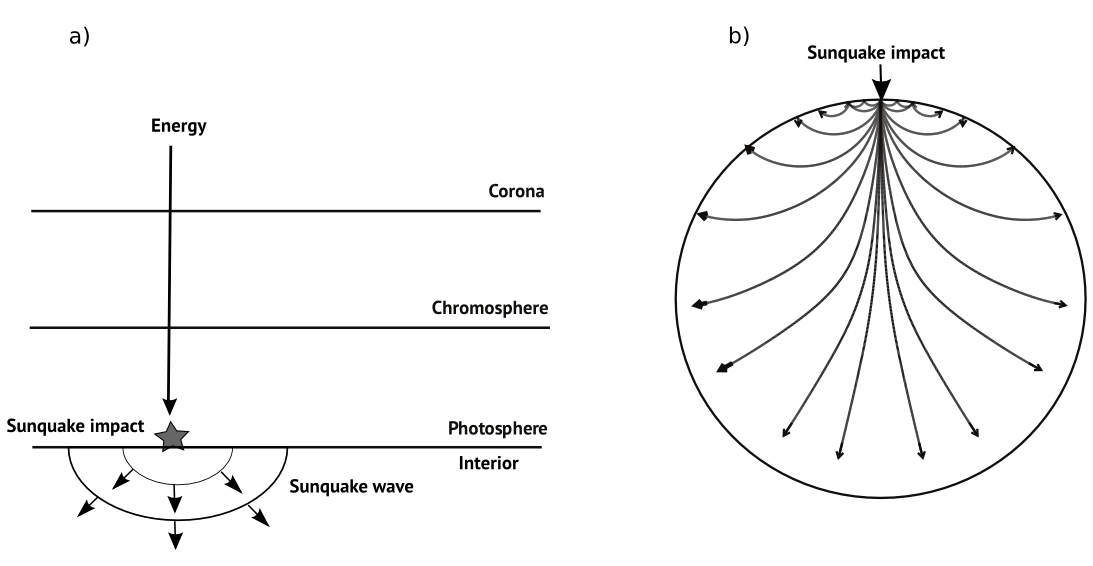
\includegraphics[width=0.99\textwidth]{sunquake-cartoon}
  \caption{Sunquake cartoon: a) Shows how energy and momentum must traverse through the solar atmosphere before impacting the photosphere to generate a sunquake. b) Shows acoustic wave-fronts propagating into the interior of the Sun. Wave-fronts refract back toward the surface as they encounter increasingly dense sub-surface layers. Waves reaching the surface disturb material in a pattern resembling ripples in a pond. Courtesy of \cite{2014arXiv1402.1249K}}\label{sunquake-cartoon}
\end{center}
\end{figure}


\subsubsection{Sunquake Generation}\label{sunprog}
%list and explain current theories of sunquake generation
%making sure to highlight the different observables that can identify each mechanism, eg wlf = evidence of radiative backwarming


The progenitors of sunquakes are still unknown and as a result this is an exciting area of research with discoveries still to be made. The general consensus, in terms of valid mechanisms that could cause this phenomenon is an area of contention, however the following progenitors are thought to be at least partly responsible. Each mechanism is associated with different observable signatures of which each observed sunquake may have some, none or many. This means that a rigid description of the transport of flare energy and momentum to the sub-photosphere is probably unlikely. Instead each candidate progenitor may play a bit part in the process, and there very well maybe mechanisms yet undiscovered. \\

\begin{itemize}
\item \textbf{Radiative backwarming} as a mechanism for producing sunquakes, was first put forward by \cite{2005ApJ...630.1168D} to account for a spatial correlation between seismic sources and white light emission from the lower atmosphere. During a solar flare, high energy electrons and photons impulsively heat the chromosphere and photosphere leading to an enhancement in white light emission \citep{1989SoPh..124..303M}. This WL enhancement can be generated by either; Balmer continuum generated by hydrogen bound-free emission in the upper-chromosphere, which irradiates the photosphere increasing local plasma temperature; $H^{-}$ emission at deeper altitudes, near the temperature minimum region. In both cases, an impulsive increase in radiation pressure and gas pressure exerted on the photosphere could generate acoustic waves which propagate into the sub-photosphere. Therefore a clear radiative energy contribution from Balmer continuum and general white light emission are considered signatures of radiative backwarming. For backwarming to be responsible for the sunquake, a comparable radiative energy budget in a Balmer or white-light signature would be required.\\

\item \textbf{Sudden magnetic field reconfiguration} was first detailed by \cite{2008ASPC..383..221H}. Solar flares are violent physical processes dictated by the interplay between reconnecting magnetic fields and charged solar plasma.
If the magnetic field close to the photosphere relaxes to a more horizontal alignment it can impart a Lorentz force on the local plasma environment, resulting in the production of acoustic waves in the sub-photosphere. The key parameter for this mechanism seems to be that the field has to reconfigure in an sufficiently impulsive manner to generate enough force to induce seismic waves. An observable signature of this progenitor would be impulsive changes in magnetic field strength close to the sunquake. \\

\item \textbf{Shocks} are a mechanism originally proposed in initial work by \cite{1995ESASP.376b.341K} and \cite{1998Natur.393..317K}, whereby a shock wave propagates from the upper-chromosphere down to lower altitudes. During a solar flare, particles and heat are directed down toward the chromosphere, at which point chromospheric material reacts by increasing in temperature. This increased temperature causes explosive ablation of chromospheric material both upward and downward. The downward component develops into a shock front carrying energy to the lower atmosphere, which can go on to impact the photosphere generating acoustic waves. If the shock is dissipated at higher altitudes such as the lower chromosphere, heat generated during the deposition process can irradiate the photosphere with high energy photons, causing radiative backwarming \citep{1989SoPh..124..303M}. If the sunquake is caused by a shock then acoustic impacts should occur approximately 100 seconds after the HXR signature associated with the flare impulsive phase, as dictated by the thick target model. Observational signatures of shocks are red or blue shifted wavelengths which can be captured in Dopplergrams or spectroscopic data. \\

\item \textbf{Direct particle collision}, is linked to early work by \cite{1998Natur.393..317K} and observations by \cite{2007ApJ...664..573Z} where the sunquake was spatially aligned with HXR and $\gamma$-ray emission respectively. HXRs are due to the presence of a nonthermal accelerated electron beam giving up collisional energy to the chromosphere. Whereas $\gamma$-rays during a solar flare are an indicator of energetic protons being accelerated along a newly reconfigured magnetic field. Proton beams carry more momentum than electron beams and are able to penetrate through the solar atmosphere to lower altitudes, therefore being more likely to cause a sunquake. If an nonthermal beam of electrons or protons makes it down to the photosphere, it can deposit energy in the form of an acoustic impact which propagates into the subphotosphere. HXRs and $\gamma$-rays are both observable by the Ramaty High Energy Solar Spectroscopic Imager (RHESSI), see section \ref{rhessi}. \\

\end{itemize}
%It is also theoretically possible to heat the upper photosphere by resistive dissipation of Alfven waves \citep{1982SoPh...80...99E}


\subsubsection{Local Helioseismology}
%use content from old report...maybe expand a little
Helioseismology is a tool for probing the interior of the Sun. Most techniques in this field of analysis rely on observations of gravity and acoustic waves on the photosphere that are the result of interior excitation. Studying the frequency and modes of these oscillations has revealed much about the internal structure of the Sun. Local helioseismology is a collection of techniques developed for global helioseismology that have been modified for use in studying local regions in higher spatial resolution. The following section provides an introduction to some of these techniques.


\paragraph{Helioseismic Holography}\label{helioholog}
\cite{1999ApJ...513L.143D} pioneered the use of helioseismic holography to produce seismic images of the solar flare of July 1996 reported to have a sunquake by Kosovichev and Zharkova. Time series egression-power maps at 3.5 and 6 mHz were computed with a 2 mHz bandwidth. It was found that the most powerful acoustic power frequency associated with the flare is centred at 3.5 mHz but has a large amount of noise. However, the 6 mHz range has a much lower ambient noise, therefore producing a better rendering of the seismicity of the flare. It is now standard practice to use the 6 mHz range for helioseismic holographic calculations of egression-power. \\
Originally the idea of analysing Doppler images of the solar surface in order to observe acoustic sources was put forward by \cite{1975CRASB.281...93R}. Helioseismic holography was developed further in concept by Lindsey and Braun \citep{1990SoPh..126..101L, 1992ApJ...392..739B, 1997ApJ...485..895L} in an effort to to image the solar interior and far-side of the Sun. This technique involves using a Doppler image of a location on the solar surface as a reference wave-field to enable an estimation of that wave-field at a location in the solar interior at a time preceding or proceeding the image. This is achieved by calculating the ingression or egression of the wave-field by assuming that it's evolution is a, convergence to, or divergence from, the point of origin of that wave-field. The technique uses Green's function (eqn \ref{green}, where $\vec{r}$ and $t$ are position and time of an observed signal and $\vec{r}'$ and $t$' are the position and time of the signal earlier in time) which assumes that the acoustic wave propagates from a point source, allowing a signal $\psi(\vec{r},t)$ observed on the surface to be devolved backwards in time.

\begin{equation}\label{green}
G_{+}(|\vec{r}-\vec{r}'|,t-t')
\end{equation}

Where $a$ and $b$ constrain the holographic pupil, equation \ref{holog} is then used to devolve the surface signal to calculate the position of subsurface acoustic sources.

\begin{equation}\label{holog}
H_{+}(\vec{r},z,t)= \int dt'  \int_{a<|\vec{r}-\vec{r}'|<b} d^{2}\vec{r}'G_{+}(|\vec{r}-\vec{r}'|,t-t')\psi(\vec{r}',t')
\end{equation}

Equation \ref{eggpower} is then used to calculate the egression power associated with the acoustic sources at a time $t$.

\begin{equation}\label{eggpower}
P(z,\vec{r})=\int dt|H_{+}(\vec{r},z,t)|^{2}dt
\end{equation}

If egression power is required in terms of frequency then equation \ref{eggpower} can be Fourier transformed into frequency space.


\paragraph{Time-Distance}\label{TD}
The first observation of a sunquake \citep{1998Natur.393..317K} used the time-distance technique to track sunquake wavefronts. The paper by \cite{1993Natur.362..430D} explains how to extract time-distance (TD) information from observations of intensity fluctuations on the solar surface. This technique uses travel times of waves between two locations on the solar surface. The method assumes that the travel time of a wave propagating in the interior of the Sun will be modified by any anomalies that it has to travel through, thus the resulting signal will contain the signatures of those irregularities. For instance, if the wave encounters a flow along it's path of travel, it will propagate faster with the flow than against it, affecting travel time.
This technique remaps Dopplergrams into polar coordinates, with the point of origin centred on the area of downflowing material during the flare. This remapped image is then Fourier transformed with respect to azimuthal angle, with the resulting image highlighting circular disturbances as a line of positive slope.

\subsubsection{Sunquake Literature Review}
The idea that solar flares can cause acoustic waves inside the Sun was originally put forward by \citep{1972ApJ...176..833W}. Wolff made the connection that a large solar flare releasing enough energy to heat the photosphere, would generate expansion of photospheric material, which could lead to an impulsive stimulation of oscillations in the Sun's interior. Wolff also commented that it would be difficult to observe interior oscillations with current (in the 1970s) solar velocity measurement techniques.

A little over twenty years later and Wolff's idea was built upon by \cite{1995ESASP.376b.341K}, who showed theoretically that acoustic waves in the solar interior could be generated by a large solar flare, and that they may be detectable. A year later and the first detection of a sunquake was made by \cite{1998Natur.393..317K} during an X class solar flare on July the 9th 1996. Their observational data came from the Solar and Heliospheric Observatory (SOHO) via the Michelson Doppler Imager (MDI) which images the movement of photospheric material by analysing shifts in wavelength of the emitted light. They observed a prominent impulsive downward signature in the Dopplergrams directly over a compact point source which subsequently emanates a set of concentric acoustic waves (see Figure \ref{mdiquake96}). The timing of maximum downward velocity of material derived from the Dopplergrams was out of sync with peak hard x-ray measurements by around a minute. This time delay, coupled with white-light enhancement in the lower atmosphere led to the conclusion that during the flare, accelerated energetic particles heat the cool dense chromosphere causing a shock front which travels downward, depositing energy in lower atmospheric layers, generating a sunquake.

\begin{figure}[hb]
  \begin{center}
  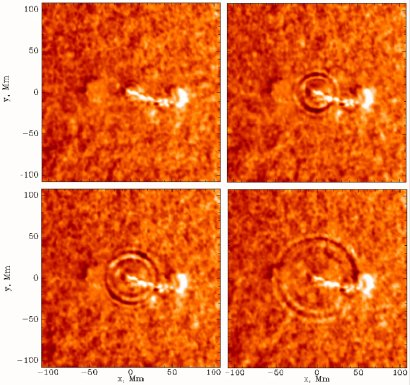
\includegraphics[width=0.80\textwidth]{soho-mdi-quake-96}
\caption{\cite{1998Natur.393..317K} produced SOHO MDI Dopplergrams of the photosphere from the 1996 July 9th, X class solar flare showing the sunquake expanding outward from it's seismic epicentre to a radial distance of $1.2\times10^{8}$ metres. Wave-fronts accelerate from a velocity of 30km/s to 100km/s}\label{mdiquake96}
\end{center}
\end{figure}

The first sunquake observation opened up a whole new area of solar physics, leading to subsequent detections associated other flares. The majority of observations show that sunquakes are often the product of highly impulsive flares, with the acoustic source aligning spatially with white light enhancement in the lower solar atmosphere and hard x-ray emission in the upper-atmosphere \citep{2005ApJ...630.1168D, 2007ApJ...664..573Z}. \cite{2005ApJ...630.1168D} went on to calculate the energy needed to stimulate the propagation of an acoustic wave in the sub-photosphere, finding that only $\sim10^{-3}$ of the energy released by a flare is enough to generate a sunquake. This was an important calculation because it forced the solar community to consider that it might be possible for low energy flares to produce sunquakes, leading to subsequent work by \cite{2008SoPh..251..613M} looking at seismicity of M-class flares.

A paper by \cite{2000ApJ...531L..75H} put forward for the first time, that sunquake production may depend on the changing configuration of the local magnetic field. This idea was further reinforced by \cite{2001ApJ...550L.105K} reporting observations of impulsive changes in magnetic field strength at the photosphere during a solar flare. These magnetic transients were shown to approximately correlate in time and space with hard x-rays, impulsive increases in plasma velocity and increased emission. This line of study was continued \citep{2009MNRAS.395L..39M}, investigating the magnetic field variation of the photosphere in many flares. The study found that some flares with seismicity do not have a spatial and temporal correlation between sunquakes and magnetic transients. Some flares have magnetic transients and no seismicity, and some flares have a good co-spatial alignment of acoustic activity and magnetic variability. It was noted that the impulsiveness of the magnetic field variation could be important as to whether a sunquake is generated.

Some of the most intriguing of sunquake observations are those that do not abide by the usual set of observable features, in that they are not necessarily associated with hard x-rays and excess white-light emission. For example, a statistical survey carried out by \cite{2012SoPh..277..317P}, highlighted a flare containing three footpoints with a seismic source that was co-temporal but not co-spatial with it's closest HXR footpoint; and another source which was co-spatial and co-temporal with its nearest HXR footpoint. This showed that a sunquake does not necessarily correlate with locations of peak emission. Another example by \cite{2011ApJ...741L..35Z} reports an observation of two seismic sources associated with footpoints of an erupting flux rope. During the eruption, the magnetic field above each seismic source undergoes an abrupt permanent reconfiguration. The authors cite the possibility that there exists particle beams low enough in population that HXR emission is undetectable. Further papers investigating the same event \cite{2013SoPh..284..315Z} show that there are downward motions of material above the seismic sources and that energy provided by magnetic transients may not be able to account for the acoustic power generated. These observational oddities prove that mechanisms that generate sunquakes are not well understood and there is much research to be done to classify the different progenitors. For instance, \cite{2014ApJ...796...85J} tests multiple sunquake progenitors observationally, finding that there is no obvious signature to back up any of the current theories. Based on the same event, \cite{2015ApJ...812...35M} find that the sunquake is probably due to a hydrodynamic response resulting in a downward propagating shock wave. This is due to strong red-shifted signal over the acoustic source at the correct time. \cite{2015IAUGA..2286139S} report a sunquake associated with a flare that does not have an erupting filament and lacks a hard x-ray signal that spatially aligned with the acoustic source. This means that not only is the eruptive flare model not governing the flare but also the sunquake is not caused by a particle beam. They suggest that electric currents the photospheric magnetic field may have the energy and impulsiveness required to produce an acoustic response. This is because the highest calculated radial currents partially correlate with the sunquake location. Electric currents as sunquake generator is not considered in this work but will no doubt be included in future projects (see Project 2 in Section \ref{thesisplan}). More recently, work follows suit showing that a sunquake associated with a low power C-class flare that could be caused by dissipation of electric current or Lorentz force in the lower atmosphere \citep{2015ApJ...807..102S}. In this case, the sunquake is formed at a time coinciding with emission from nonthermal electrons but the HXR signature is not aligned with the acoustic source. Instead, the sunquake is spatially aligned with fast changing magnetic field lines, leading to the impulsive generation of strong electric currents. The most recent sunquake paper \citep{2016arXiv160208245R} approaches the problem of acoustic wave production in the photosphere from a theoretical model of coronal magnetic field configuration. The work simulates different movements of coronal loops and finds that changes in coronal magnetic field do indeed propagate to the lower atmosphere with enough Lorentz force to create a sunquake.

  



